\documentclass[12pt,oneside,notitlepage,abstracton,a4paper]{scrartcl}
\usepackage{epsfig,scrpage2,graphicx,subfig}
\usepackage{float}
\usepackage{hyperref}
\usepackage{listings}
\usepackage{csquotes}

\setcounter{secnumdepth}{3}

\setlength{\parindent}{1.5em}
\usepackage{indentfirst}
\setlength{\parskip}{0ex plus0.5ex minus0ex}
\pagestyle{scrheadings}
\bibliographystyle{unsrt} 
\captionsetup[figure]{font=small,skip=0pt}

\renewcommand{\headfont}{\normalfont}

\cfoot{\pagemark}

% A picture on top of the titlepage
\subject{
\includegraphics[height=2cm]{pics/knu} 
\includegraphics[height=2cm]{pics/desy} 
\includegraphics[height=2cm]{pics/lpnhe}}

\title{\Large TCT-Analysis Framework Developers Guide} 
\author{ Mykyta Haranko \\ \normalsize Taras Shevchenko National University of Kyiv, Ukraine \\ \footnotesize mykyta.haranko@gmail.com }

\date{\normalsize \today}

\begin{document}

\maketitle

\begin{abstract}

\noindent
This guide was written for users and developers of the TCT-Analysis framework to understand basic aspects of the program and to make them able to extend its functionality for further data analysis.
\end{abstract}

\newpage
\tableofcontents
\newpage 

\section{Introduction}\label{intro}

The Transient Current Technique (TCT) is widely used for studying the detector response after high irradiation fluences. The main idea is to use laser to produce charge carriers in the sensor, which is similar to the energy loss process of a minimum ionizing particle crossing the detector\cite{bib:haranko_desy}. Then waveforms are stored in a binary files and processed using different methods.
\\ \indent TCT-Analysis is a framework proposed by Hendrik Jansen and developed to make the data analysis process fast and unified for all the laboratories using this technique. The basic idea was to create one open source framework, to which people can easily add their analysis and share it with other people.

\section{Usage}\label{usage}

This section gives simple instructions on downloading, installation and usage of the framework, also gives a brief description of the configuration file.

\subsection{Downloading and Installation}\label{usage:installation}

There are two options available - console and graphical version of the framework. User can download pre-compiled Windows version or compile it from source.

\subsubsection{Pre-compiled version}

The pre-compiled version is distributed only for Windows, for other operating systems it has to be compiled from source. TCT-Analysis requires ROOT 5.34.XX to be installed. Download needed version from \url{https://root.cern.ch/} and add it to the PATH environmental variable (usually offered by ROOT installer).
\\ \indent The next step is downloading the latest release of the framework from:
\begin{displayquote}
\url{https://github.com/garankonic/TCT-analysis/releases}
\end{displayquote}
Windows pre-compiled versions are stored in *.zip file. To install the program one needs to unzip the archive to the desired directory.
To start the program run \textbf{TCT-Analysis-QT.exe} in the \textbf{TCT-Analysis/bin} folder.
\\ \indent The last release was linked against ROOT 5.34.32. Tested on Windows 7, Windows 8.1 with ROOT 5.34.XX. Compiled using msvc2013 compiler.

\subsubsection{Compiling from source using CMake}

To compile the framework from source using CMake next prerequisites have to be satisfied:
\begin{itemize}
\item ROOT 5.X or 6.X has to be installed, ROOTSYS variable has to be defined.
\item CMake 2.6 or older has to be installed and added to PATH variable.
\item (if GUI needed, \textbf{recommended}) Install Qt4 (Qt5 building with CMake not implemented for the moment).
\item (optional, for single waveforms acquisition) If LeCroy RAW data files converter needed - put the external LeCroyConverter lib to the \textit{external/LeCroyConverter/lib/libLeCroy.so}.
\end{itemize}

After satisfying dependencies, follow next steps for both Windows and Linux operating systems:
\begin{enumerate}
\item Checkout the latest release of the program from the Github repository:
\begin{displayquote}
\url{https://github.com/garankonic/TCT-analysis/releases}
\end{displayquote}
Or go to the master branch to get the latest version in development
\begin{displayquote}
\url{https://github.com/garankonic/TCT-analysis}
\end{displayquote}
\item Go to the \textbf{TCT-Analysis/build} directory.
\item Run "\textbf{cmake $\langle$options$\rangle$ ..}" command with the next available options.
\begin{enumerate}
\item \textbf{-DWITH\_GUI=ON} -- compiles GUI version of the framework. Default -- OFF.
\item \textbf{-DWITH\_LECROY\_RAW=ON} -- links against LeCroyRAW Converter library. Default -- OFF.
\end{enumerate}
\item Run \textbf{make install}.
\item Go to the \textbf{TCT-Analysis/bin} directory.
\item Run \textbf{tct-analysis} or \textbf{tct-analysis.exe} executable.
\end{enumerate}

\subsubsection{Compiling from source using qmake}

To compile the framework from source using qmake next prerequisites have to be satisfied (compilation with GUI):
\begin{itemize}
\item ROOT 5.X or 6.X has to be installed.
\item Install Qt4 or Qt5.
\end{itemize}

After satisfying dependencies, follow next steps for both Windows and Linux operating systems:
\begin{enumerate}
\item Checkout the latest release of the program from the Github repository:
\begin{displayquote}
\url{https://github.com/garankonic/TCT-analysis/releases}
\end{displayquote}
Or go to the master branch to get the latest version in development
\begin{displayquote}
\url{https://github.com/garankonic/TCT-analysis}
\end{displayquote}
\item Open \textbf{TCT-Analysis.pro} file in \textbf{Qt Creator}.
\item Follow instructions to configure compilation of the program.
\item Change \textbf{TCT-Analysis.pro} file according to the location of ROOT libraries and include files.
\item Press \textbf{Ctrl+B} to build the program.
\item Repeat previous steps for \textbf{tbrowser.pro} file to compile \textbf{TBrowser}.
\item Both executables (\textbf{tct-analysis} and \textbf{tbrowser}) has to be placed in the \textbf{TCT-Analysis/bin} folder. 
\item Create \textbf{default.conf} file in \textbf{TCT-Analysis/bin} folder containing:
\begin{displayquote}
DefaultFile = ../testanalysis/lpnhe\_top.txt
\end{displayquote}
\item Run the program. Note: be sure that Qt libraries are present in the PATH variable (LD\_LIBRARY\_PATH for Linux) or in the execution folder, otherwise program may fail to start, the same is for ROOT libraries.
\end{enumerate}

\subsection{First Run}\label{usage:first_run}

The following folder structure is present in the base folder:
\begin{itemize}
\item \textbf{./bin} -- contains executables and linked libraries
\begin{itemize}
\item \textbf{./bin/default.conf} -- contains name of the config file loaded by default
\item \textbf{./bin/execution.log} -- log file of the program execution and data analysis
\item \textbf{./bin/tct-analysis.exe} -- execution of the program
\item \textbf{./bin/tbrowser.exe} -- TBrowser execution
\end{itemize}
\item \textbf{./results} -- here program stores output data by default
\item \textbf{./testdata} -- folder with test data, contains one data file with focus search at “lpnhe” folder
\item \textbf{./testanalysis} -- folder with sample program configuration files
\item \textbf{./testsensor} -- folder with sample sensor configuration files.
\end{itemize}
Depending on the selected options of compilation from Section~\ref{usage:installation} user can have either console or graphical version of the program.
\\ \indent In case of the console version of framework, file with configuration has to be specified: 
\begin{lstlisting}
./tct-analysis -af <path-to-configuration-file> 
\end{lstlisting}
for example 
\begin{lstlisting}
./tct-analysis -af ../testanalysis/lpnhe_top.txt
\end{lstlisting}

\indent In case of the graphical version, configuration file specified in \textbf{bin/default.conf} will be loaded by default. In Figure~\ref{fig:main} main window of the program is shown.

\begin{figure}[H]
    \centering
    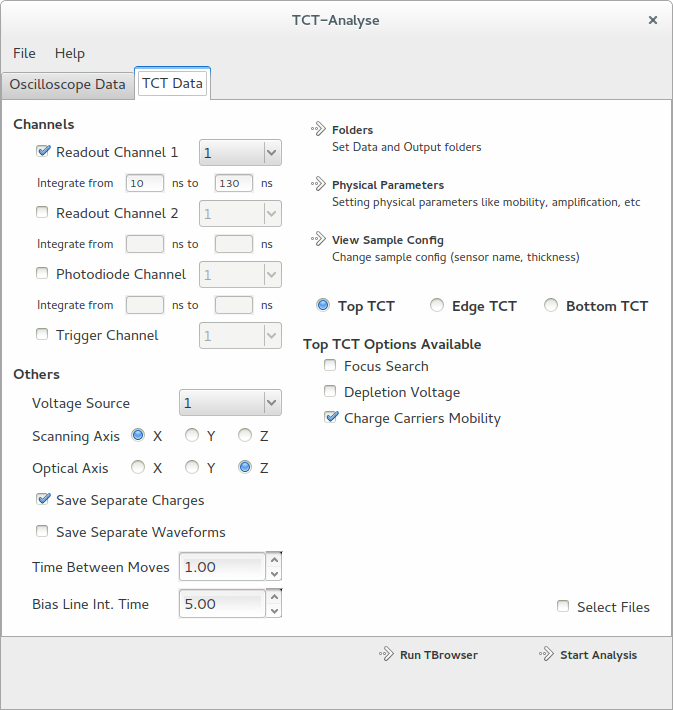
\includegraphics[width=8cm]{pics/main_window}
    \caption{Main window of the framework graphical version.}
    \label{fig:main}
\end{figure}

\indent To Open/Save new configuration file follow the corresponding file dialogue in the \textbf{File} menu at the top.
\\ \indent In Figure~\ref{fig:main_structure} structure of the main window explained with key control elements signed. 

\begin{figure}[h]
    \centering
    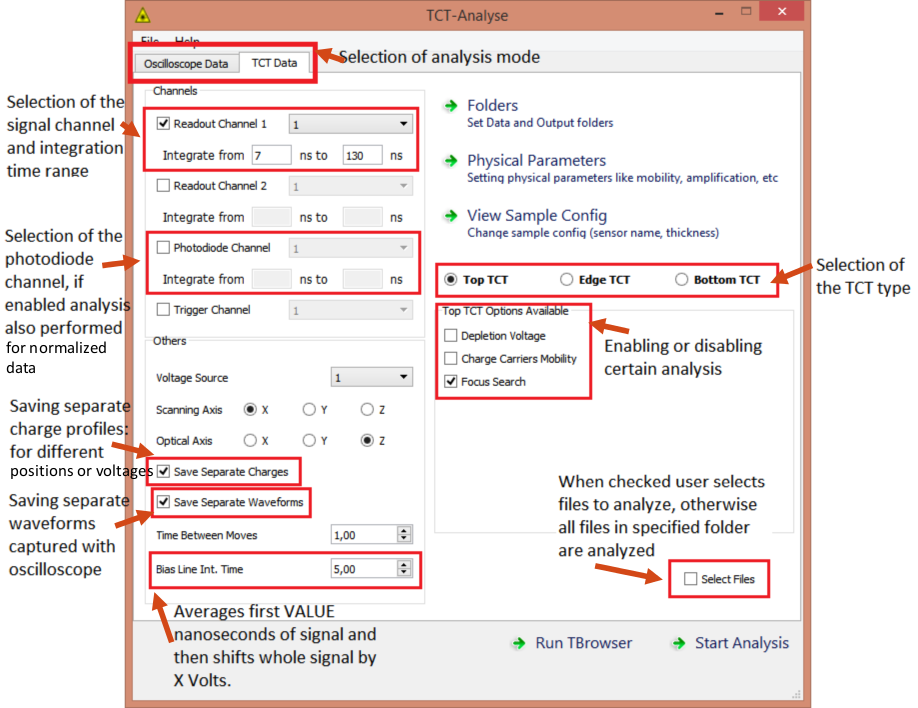
\includegraphics[width=18cm]{pics/main_structure}
    \caption{Structure of the main window.}
    \label{fig:main_structure}
\end{figure}

\begin{itemize}
\item To change data folder or output folder press \textbf{Folders} button.
\item \textbf{Physical Parameters} button is used to set physical quantities used for certain analysis.
\item \textbf{View Sample Config} used to change sensor name, thickness or general sensor configuration file.
\item \textbf{Run TBrowser} button is used to view output root files with analysed data.
\item To run analysis click \textbf{Start Analysis} button. If \textbf{Select Files} is checked one need to select *.tct data file to analyse, otherwise all data files in the specified folder analysed.
\end{itemize}

Normally for the graphical version user don't have to interact with the configuration *.txt file, but in case of the console version, configuration files are saved with comments, explaining all the parameters. Example of the configuration file is attached in Appendix~\ref{App:conf}.
\\ \indent 

\subsection{Sample Data File}\label{usage:sample}



\clearpage 
\appendix
\section{Sample configuration file}\label{App:conf}

Here sample TCT-Analysis configuration file is presented. Follow the comments to understand logic.
\begin{lstlisting}[
    basicstyle=\tiny, %or \small or \footnotesize etc.
]
#comments have to start with a
#put group key words in []
#always specify ID, TAB, "=", TAB, value

[General]
ProjectFolder	=	./
DataFolder	=	../testdata/lpnhe
Outfolder	=	../results/

#Set acq mode.
# 0 - taking the sets of single measurements (*.txt or *.raw files by oscilloscope). Settings are in [Analysis]
# 1 - taking the data from *.tct file produced by DAQ software. Settings are in [Scanning]
Mode	=	1

[Analysis]
MaxAcqs	=	100
Noise_Cut	=	0.005
NoiseEnd_Cut	=	0.005
S2n_Cut	=	3
S2n_Ref	=	2
AmplNegLate_Cut	=	-0.02
AmplPosLate_Cut	=	0.015
AmplNegEarly_Cut	=	-0.02
AmplPosEarly_Cut	=	0.02
DoSmearing	=	0
AddNoise	=	0
AddJitter	=	0
SaveToFile	=	1
SaveSingles	=	1
PrintEvent	=	4294967295
LeCroyRAW	=	0

[Scanning]
#Channels of oscilloscope connected to detector, photodiode, trigger. 
#Put numbers 1,2,3,4 - corresponding to channels, no such device connected put 0.
CH_Detector	=	1
#Turning on of the Photodiode channel also adds normalisation to all scans
CH_Photodiode	=	0
CH_Trigger	=	0
#Set optical Axis. 1-x,2-y,3-z
Optical_Axis	=	3
#Set scanning Axis. 1-x,2-y,3-z
Scanning_Axis	=	1
#Set voltage source number (1 or 2)
Voltage_Source	=	1
#Time between stage movements in seconds.
Movements_dt	=	1
#Set the integration time in ns to correct the bias line. 
#Program averages the signal in range (0,value) and then shifts the signal by the mean value.
CorrectBias	=	5
#Perform next operations. Analysis will start only if all needed data is present:
# 0-top,1-edge,2-bottom
TCT_Mode	=	0

#Scanning over optical and perpendiculr to strip axes 
#(or along the detector depth in case of edge-tct), fitting the best position.
Focus_Search	=	0
#Depletion Voltage
EdgeDepletionVoltage	=	1
#Electric Field Profiles
EdgeVelocityProfile	=	1
#Averaging the current for electric field profile from F_TLow to F_TLow+EV_Time
EV_Time	=	0.3
#Depletion Voltage
TopDepletionVoltage	=	0
#Charge Carriers Mobility
TopMobility	=	1

#Integrate sensor signal from TimeSensorLow to TimeSensorHigh - ns
TimeSensorLow	=	10
TimeSensorHigh	=	130
#Integrate photodiode signal from TimeDiodeLow to TimeDiodeHigh - ns
TimeDiodeLow	=	46
TimeDiodeHigh	=	51

#Save charge, normed charge and photodiode charge for each Z, voltage
SaveSeparateCharges	=	1
#Save waveforms for each position and voltage
SaveSeparateWaveforms	=	0

[Parameters]
#low-field mobility for electrons, cm2*V^-1*s^-1
Mu0_Electrons	=	1400
#low-field mobility for holes, cm2*V^-1*s^-1
Mu0_Holes	=	450
#saturation velocity cm/s
SaturationVelocity	=	1e+07
# amplifier amplification
Amplification	=	300
# factor between charge in sensor and photodiode due to light splitting: Nsensor/Ndiode
LightSplitter	=	9.65
# resistance of the sensor and diode output, Ohm
ResistanceSensor	=	50
ResistancePhotoDetector	=	50
# pohotodetector responce for certain wavelength, A/W
ResponcePhotoDetector	=	0.7
# electron-hole pair creation energy, eV
EnergyPair	=	3.61

[Sensor]
SampleCard	=	../testsensor/SC_M2015.txt
\end{lstlisting}

\clearpage

\begin{thebibliography}{99}
\begin{sloppypar}
\bibitem{bib:haranko_desy} http://www.desy.de/f/students/2015/reports/MykytaHaranko.pdf
\end{sloppypar}
\end{thebibliography}

\end{document}
